\documentclass[11pt]{article}
\usepackage{url,graphicx,tabularx,array,amsmath,amssymb,amsthm,booktabs,float}
\usepackage[margin=.65in]{geometry}
\setlength{\parskip}{1ex} %--skip lines between paragraphs
\setlength{\parindent}{0pt} %--don't indent paragraphs
\graphicspath{{C:/Users/Colin/Documents/GitHub/BB_data_analysis/constrained_MLE}

\DeclareGraphicsRule{.tif}{png}{.png}{`convert #1 `dirname #1`/`basename #1 .tif`.png}
\newcommand{\vcentergraphics}[2]{\ensuremath{\vcenter{\hbox{\includegraphics[#1]{#2}}}}}


%-- Commands for header
\renewcommand{\title}[1]{\textbf{#1}\\}
\renewcommand{\line}{\begin{tabularx}{\textwidth}{X>{\raggedleft}X}\hline\\\end{tabularx}\\[-0.5cm]}
\newcommand{\leftright}[2]{\begin{tabularx}{\textwidth}{X>{\raggedleft}X}#1%
& #2\\\end{tabularx}\\[-0.5cm]}


\begin{document}


\line
\leftright{10.21.16}{Colin Lewis-Beck} %-- left and right positions in the header

\begin{description}
\item \textit{Getting Proper Standard Errors From R Stan:}\\
The Hessian Stan's optimization program returns, results in a covariance matrix in terms of:
\begin{align*}
[\log(t_{p_1}),\log(t_{p_2}),\log(\sigma_1), \log(\sigma_2), p]
\end{align}

Let's use the $\Delta$ method to get a covariance matrix for: [$ \mu_1,\mu_2,\sigma_1,\sigma_2,p$].  Not the following three relationships between $\mu$ and the quantiles.

\begin{equation*}
\begin{align}
\Phi^{-1}_{SEV}(p) &=\log(-\log(1-p)) \\
\log(t_{pi})&=\mu_i +\log(\sigma_i)\Phi^{-1}_{SEV}(p_i)\\
F(t;\mu;\sigma)&=\Phi_{SEV}\left[\frac{\log(t)-\mu}{\sigma}\right]
\end{align}
\end{equation}

Solving for $\mu$ we get:
\begin{equation*}
\mu_i&=\log(t_{pi})-\exp({\log(\sigma_i)})\Phi^{-1}_{SEV}(p_i)
\end{equation}
Taking partials with respect to  $\frac{d\mu_i}{d\log(t_{pi})}$ and $\frac{d\mu_i}{d\log(\sigma_i)}$ we get:
\begin{equation*}
\begin{align}
\frac{d\mu_i}{d\log(t_{pi})} &= 1 \\
\frac{d\mu_i}{d\log(\sigma_i)} &= -\exp(\log(\sigma_i))\Phi^{-1}_{SEV}(p_i)
\end{align}
\end{equation}

It is easy to transform $\log(\sigma_i)$.  Stan estimates the SE's for p on the unconstrained space, so we use the inverse logit transformation ($\text{logit}^{-1}(p)=\frac{1}{1+e^{-p}}$) to get the SE's on the constrained space.  Putting these pieces together we get a $\Delta$ matrix:
\begin{equation*}
\begin{align}
\Delta = \begin{bmatrix}
1 & 0 & -\exp(\log(\sigma_1)\Phi^{-1}_{SEV}(p_1) & 0 & 0\\
0 & 1 & 0 & -\exp(\log(\sigma_2)\Phi^{-1}_{SEV}(p_2) & 0\\
0 & 0 & \exp(\log(\sigma_1)) & 0 & 0\\
0 & 0 & 0 & \exp(\log(\sigma_2)) & 0\\
0 & 0 & 0 & 0 & (\frac{1}{1+e^{-p}})(\frac{e^{-p}}{1+e^{-p}})\\
\end{bmatrix}
\end{align}
\end{equation}
Now, following Meeker and Escobar (Section 8.4.3), we need to get the standard errors for the GFLP CDF to make Wald bands.  Recall, the CDF: $g(\mu_1,\mu_2,\sigma_1,\sigma_2,p)=1-(1-pF(\mu_1;\sigma_1)(1-F(\mu_2;\sigma_2))$, which we can re-write as:
\begin{equation*}
\begin{align}
\Pr(t<T)&=1-(1-p\Phi_{SEV}(\mu_1,\sigma_1)(z_1))(1-\Phi_{SEV}(\mu_2,\sigma_2)(z_2))\\
&=\Phi_{SEV}(\mu_2,\sigma_2)(z_2)+p\Phi_{SEV}(\mu_1,\sigma_1)(z_1)-p\Phi_{SEV}(\mu_1,\sigma_1)(z_1)\Phi_{SEV}(\mu_2,\sigma_2)(z_2)
\end{align}
\end{equation}
Note that the SEV distribution is standardized in terms of $ z =(\log(t)-\mu)/\sigma$.  Let's again take partials of the GFLP CDF with respect to the 5 parameters.  Note: $z_1$ or $z_2$ should be plugged into the proper SEV function for each term.
\begin{equation*}
\begin{align}
\frac{dg}{d\mu_1}&=-p\phi_{SEV}(\mu_1,\sigma_1)\frac{1}{\sigma_1}+p\phi_{SEV}(\mu_1,\sigma_1)\Phi_{SEV}(\mu_2,\sigma_2)\frac{1}{\sigma_1}\\
\frac{dg}{d\mu_2}&=-\phi_{SEV}(\mu_2,\sigma_2)\frac{1}{\sigma_2}+p\Phi_{SEV}(\mu_1,\sigma_1)\phi_{SEV}(\mu_2,\sigma_2)\frac{1}{\sigma_2}\\
\frac{dg}{d\sigma_1}&=p\phi_{SEV}(\mu_1,\sigma_1)\left(\frac{-log(t)+\mu_1}{\sigma^{2}_1}\right)-p\Phi_{SEV}(\mu_2,\sigma_2)\phi_{SEV}(\mu_1,\sigma_1)\left(\frac{-log(t)+\mu_1}{\sigma^{2}_1}\right)\\
\frac{dg}{d\sigma_2}&=\phi_{SEV}(\mu_2,\sigma_2)\left(\frac{-log(t)+\mu_2}{\sigma^{2}_2}\right)-p\Phi_{SEV}(\mu_1,\sigma_1)\phi_{SEV}(\mu_2,\sigma_2)\left(\frac{-log(t)+\mu_2}{\sigma^{2}_2}\right)\\
\frac{dg}{dp}&=\Phi_{SEV}(\mu_1,\sigma_1)-\Phi_{SEV}(\mu_1,\sigma_1)\Phi_{SEV}(\mu_2,\sigma_2)\\
\end{align}
\end{equation}
Putting these into a 5 x 5 matrix we can once again use the $\Delta$ method for the standard error of g.  Then with this standard error we can use a normal approximation and get $\hat{g} \pm z_{1-\alpha/2} \hat{g_{se}}$\\\\

Taking this a step further (Meeker and Hong, p. 169) we can use a tangent method to get a CI that respects the bounds of a CDF.

Let $y_e=log(t)$.  The lower and upper bounds are calculated as:
\begin{equation*}
\begin{align*}
y_l&=y_e-\frac{z_{1-\alpha/2}\hat{g_{se}}}{\frac{dF(t)}{log(t)}}\\
y_u&=y_e+\frac{z_{1-\alpha/2}\hat{g_{se}}}{\frac{dF(t)}{log(t)}}
\end{align}
\end{equation}
Taking the derivative of the GFLP in terms of $log(t)$, which it is already parameterized in terms of is:
\begin{equation*}
\begin{align}
\frac{dg(t)}{dlog(t)}&=p\phi_{SEV}(\mu_1,\sigma_1)(z_1)(1-\Phi_{SEV}(\mu_2,\sigma_2)(z_2))(1/\sigma_1)+\phi_{SEV}(\mu_2,\sigma_2)(z_2)(1-p\Phi_{SEV}(\mu_1,\sigma_1)(z_1))(1/\sigma_2)\\
\end{align}
\end{equation}
Finally, we plug these end points back into the GFLP CDF to get our final confidence intervals.
\begin{align*}
[\hat{F}(\exp(y_l)),\hat{F}(\exp(y_u))]
\end{align}

\begin{figure}[H]
\caption{Wald Band 1 for Drive Model 3}
\centering
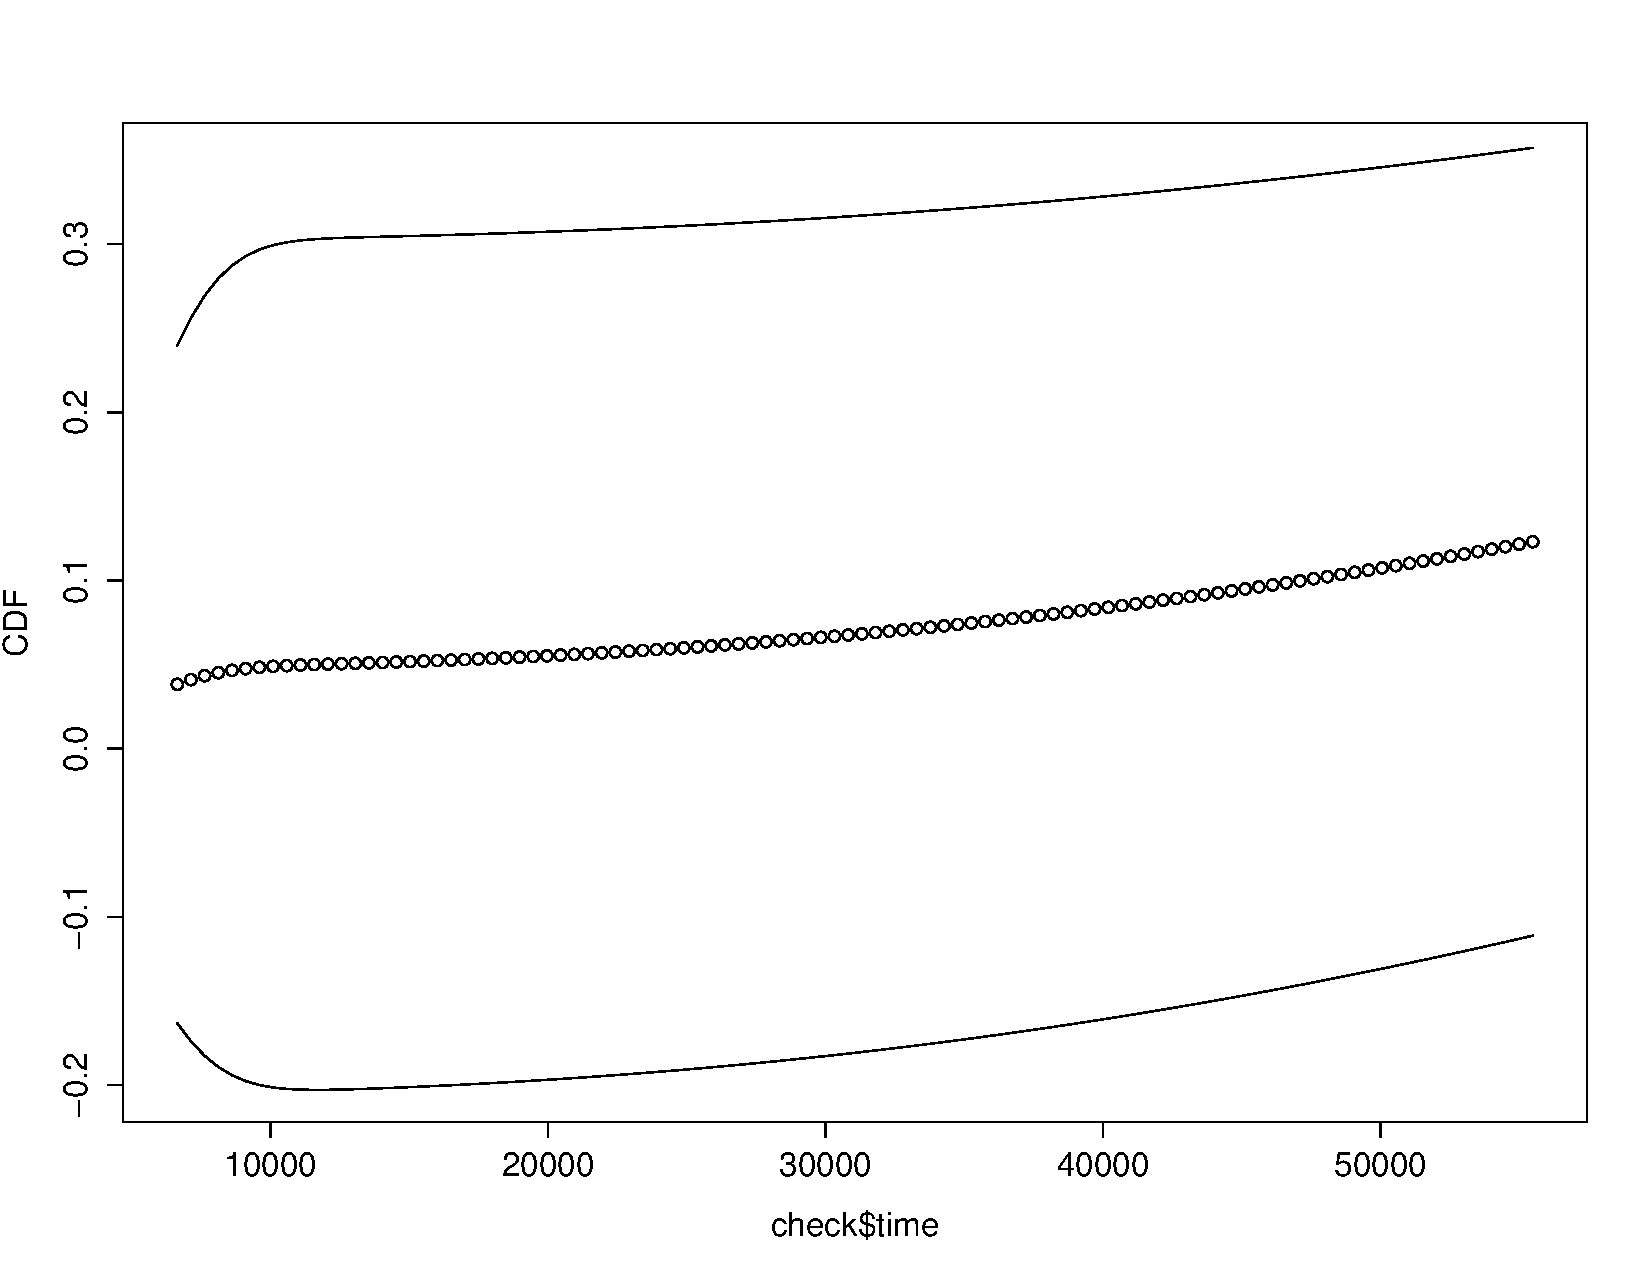
\includegraphics[height=8cm]{bandsmod3.pdf}
\end{figure}

\begin{figure}[H]
\caption{Wald Band for Drive Model 3 Hong and Meeker}
\centering
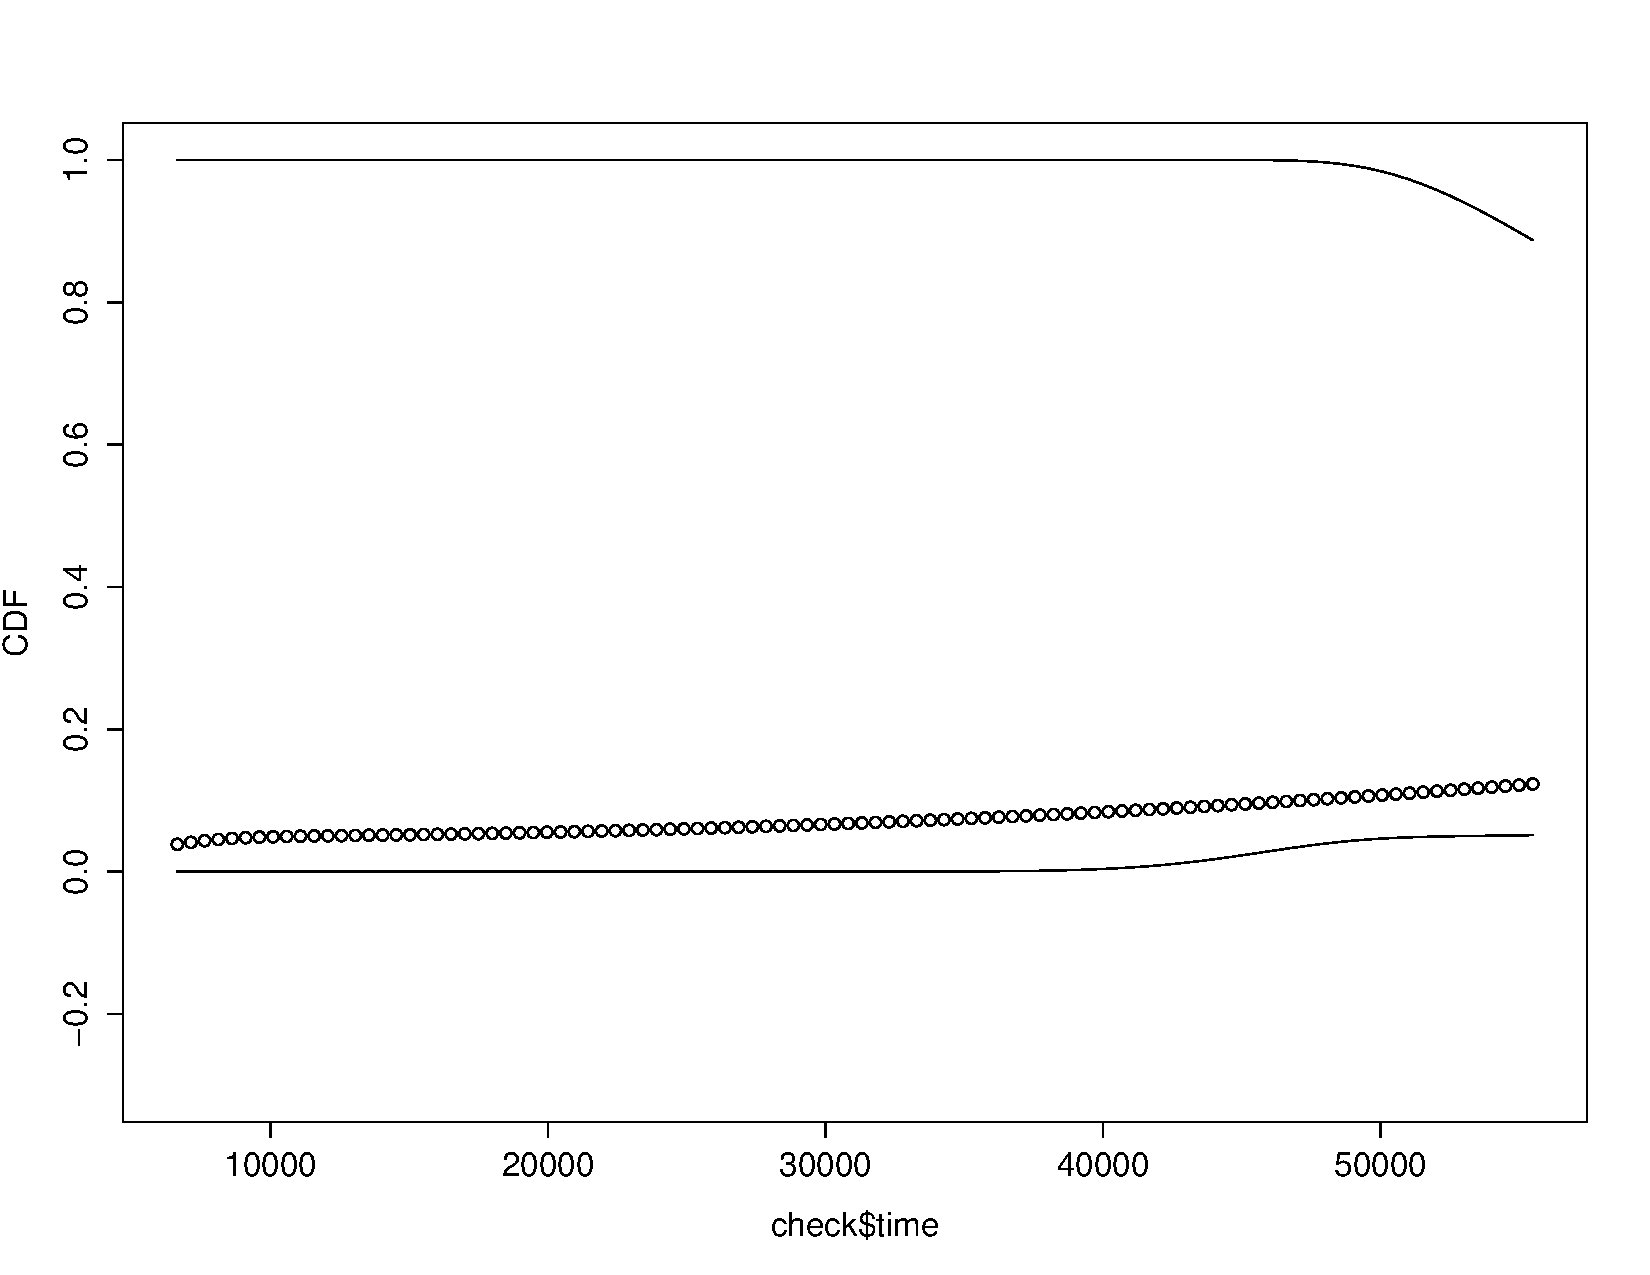
\includegraphics[height=8cm]{hongmeek.pdf}
\end{figure}



\end{document}